\subsection{M.PC.10 - Indice di stabilità dei requisiti}
\begin{figure}[H]
    \centering
    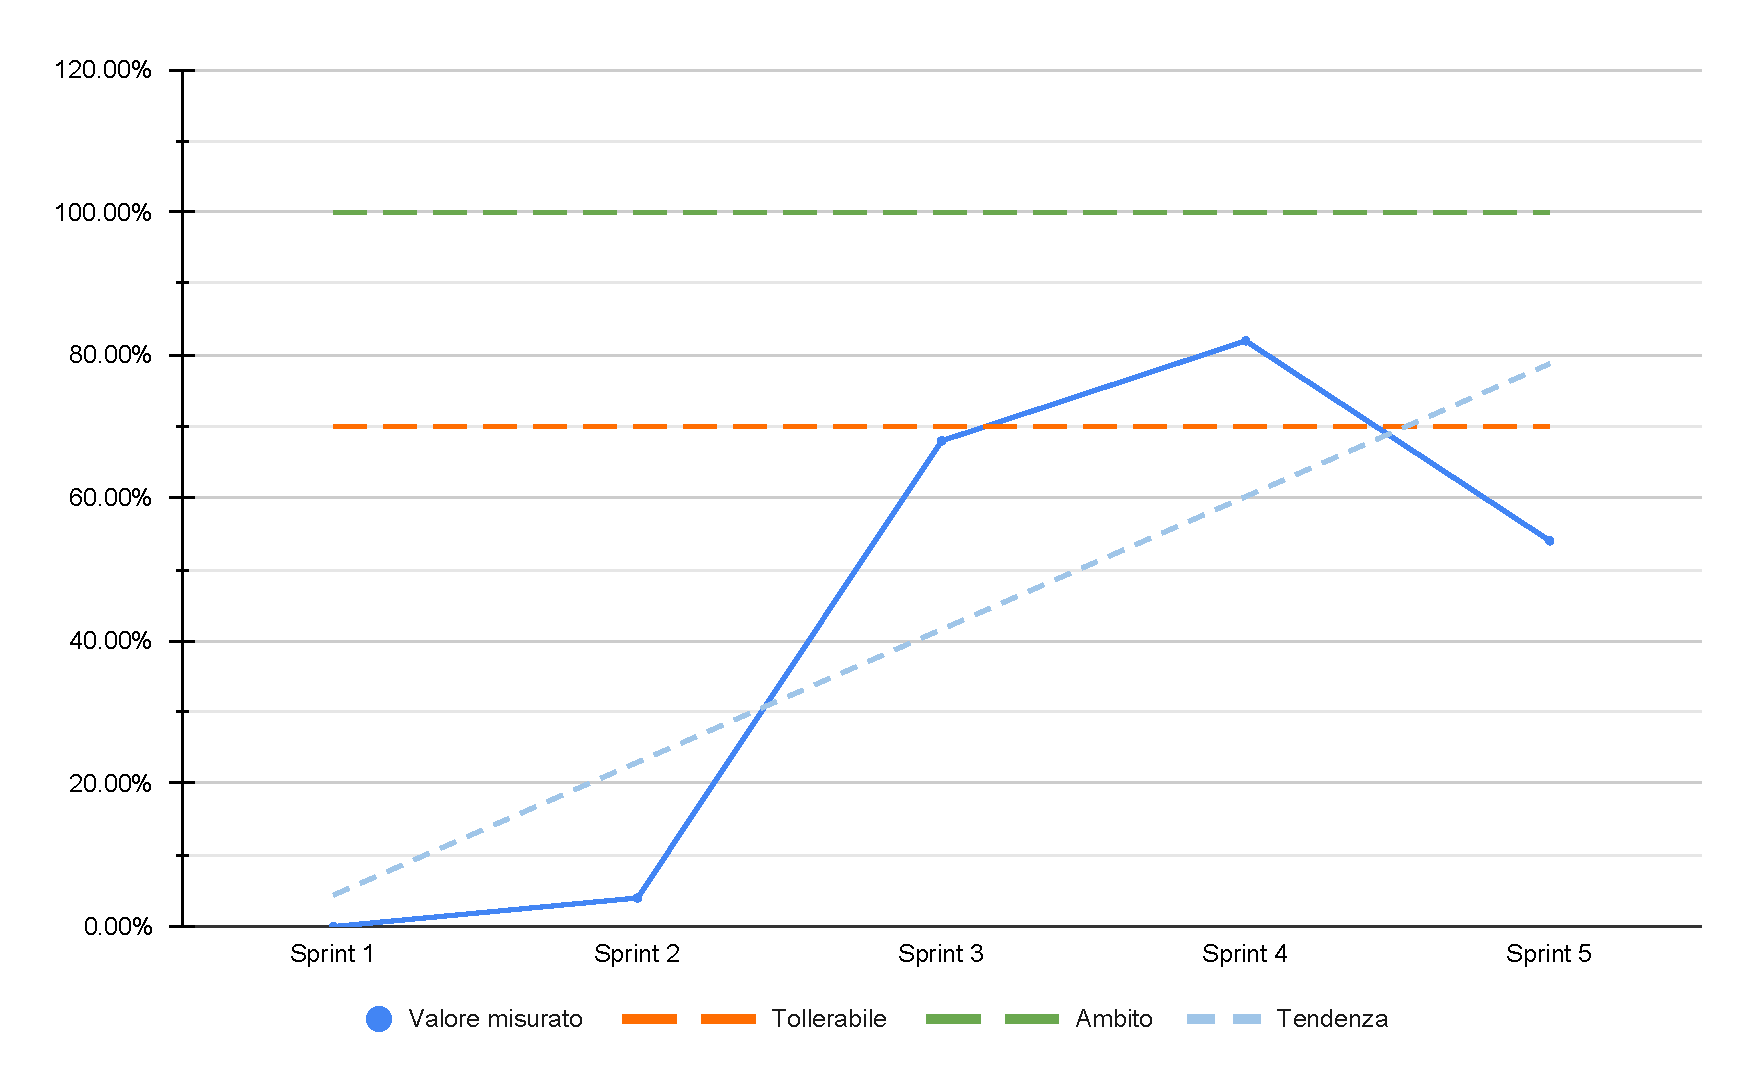
\includegraphics[width=\textwidth]{assets/stabilita_requisiti.pdf}
    \caption{M.PC.10 - Indice di stabilità dei requisiti}
\end{figure}

\par Il grafico segnala una grossa instabilità durante i primi \glossario{sprint} a causa del tracciamento iniziale dei requisiti e della creazione del documento di \AdR che ha comportato una grossa aggiunta di requisiti funzionali. Dal terzo \glossario{sprint} si nota un incremento nella stabilità causato dal minore impatto di modifiche e piccole aggiunte di casi d'uso e requisiti. Nel quinto \glossario{sprint} inizia una nuova discesa nella stabilità causata da una rivisitazione completa e l'aggiunta di casi d'uso.